\documentclass[11pt,a4paper]{article}
\usepackage[T1]{fontenc}
\usepackage[utf8]{inputenc}
\usepackage{lmodern}
\usepackage{microtype}
\usepackage[a4paper,margin=27mm]{geometry}
\usepackage[numbers,sort&compress]{natbib}
\usepackage{amsmath,amssymb,amsthm}
\usepackage{booktabs}
\usepackage{graphicx}
\usepackage[font=small,labelfont=bf]{caption}
\usepackage{xcolor}
\usepackage{hyperref}
\usepackage[nameinlink,noabbrev]{cleveref}
\hypersetup{colorlinks=true,linkcolor={blue!50!black},citecolor={blue!50!black},urlcolor={blue!50!black}}
\captionsetup[figure]{name=Fig.}
\graphicspath{{../results/figures/}}
\numberwithin{equation}{section}
\newtheorem{proposition}{Proposition}[section]
\newtheorem{theorem}[proposition]{Theorem}
\theoremstyle{remark}
\newtheorem{remark}[proposition]{Remark}
\crefname{proposition}{Proposition}{Propositions}
\DeclareMathOperator{\TV}{TV}
\DeclareMathOperator{\rank}{rank}
\DeclareMathOperator*{\argmin}{arg\,min}
\newcommand{\R}{\mathbb{R}}
\newcommand{\RR}{\mathcal{R}}
\newcommand{\NN}{\mathcal{N}}
\newcommand{\xt}{x_{\mathrm{true}}}
\newcommand{\T}{\top}

\title{Sparse-View Image Reconstruction from Radon Projections:\\ Null Space, Conditioning and Regularisation\\ of Over- and Underdetermined Systems}
\author{Xiangyu Luo\thanks{Southwest Petroleum University, Chengdu, China (\href{mailto:louang.620@gmail.com}{louang.620@gmail.com}). Course project in Scientific Computing Applications and Practice, June--July 2024.}}
\date{}

\begin{document}
\maketitle

\begin{abstract}
Parallel-beam tomography reconstructs an image from its line integrals, which after discretisation amounts to solving a linear system $Ax=b$ that is underdetermined for few projection angles and overdetermined for many. We study how the null space and the singular values of $A$, rather than the shape of the system, determine the accuracy of reconstruction methods for $100\times100$ images and 5 to 180 angles. Assembling $A$ explicitly, we compute its rank and spectrum exactly and show that every method whose output lies in the range of $A^\top$, which includes filtered back-projection (FBP), LSQR started at zero and Tikhonov regularisation, has a relative error at least equal to the fraction of the object that lies in the null space of $A$. With 10 angles 88\% of the image space is invisible, and this bound equals 0.73 for a digits phantom and 0.51 for the Shepp--Logan phantom. On data simulated on a four-times finer grid, LSQR and Tikhonov regularisation come within 0.03 of the bound, whereas total-variation (TV) regularisation solved by the Chambolle--Pock algorithm, which fills the null space with piecewise constant structure, reaches 0.25 and 0.30. With 90 and 180 angles the systems have full column rank but condition numbers of $4.3\times10^6$ and $1.4\times10^4$; the three linear methods then agree to within 0.04 and are limited by the discretisation error of the projector. At 1\% noise this error dominates the data error, makes the discrepancy principle fail unless it is included in the error estimate, and would have been concealed by the inverse crime, which overstates the accuracy of TV by up to a factor of eight. Supplementary experiments on filter windows, limited-angle data, solver convergence and computational cost show that a restricted angular range is far more damaging than a reduced number of angles, also for TV.
\end{abstract}

\noindent\textbf{Key words.} computed tomography, Radon transform, sparse-view reconstruction, ill-posed problems, null space, LSQR, Tikhonov regularisation, total variation, primal--dual methods

\smallskip
\noindent\textbf{MSC codes.} 44A12, 65F22, 65R32, 65K10, 92C55

%% ==================================================================
\section{Introduction}\label{sec:intro}

Computed tomography (CT) measures the attenuation of X-rays along many lines through an object and reconstructs the attenuation map from these line integrals, that is, from samples of its Radon transform \citep{radon1917,natterer2001}. For complete parallel-beam data the transform has an explicit inverse, and its discretisation, filtered back-projection (FBP), has been the workhorse of clinical scanners for decades \citep{kak2001,herman2009}. Clinical protocols acquire hundreds of projections, but there are strong reasons to acquire fewer: the radiation dose grows with the number of exposures, fast or dynamic imaging leaves little time per frame, and in industrial and scientific applications the geometry often restricts the accessible directions. When the number of projections falls well below what the sampling theory of the Radon transform requires, the inversion formula no longer describes the available data, and FBP reconstructions are dominated by streak artefacts.

The algebraic alternative discretises the image from the outset and treats reconstruction as the solution of a linear system $Ax=b$, in which the matrix $A$ maps pixel values to line integrals. Kaczmarz-type algebraic reconstruction techniques were among the first such methods \citep{gordon1970,andersen1984}, Krylov methods such as LSQR \citep{paige1982} solve the large sparse least-squares problems efficiently, and modern software packages collect many of these iterations \citep{hansen2018}. Because the continuous problem is ill-posed, the discrete system is ill-conditioned, and some form of regularisation, by early stopping, by a quadratic penalty or by a priori constraints, is indispensable \citep{engl1996,hansen2010,kaipio2005}. For objects that are piecewise constant, total-variation (TV) regularisation \citep{rudin1992} has proved particularly effective in sparse-view CT \citep{sidky2008}, which compressed sensing explains by the sparsity of the image gradient \citep{candes2006,jorgensen2015}, and first-order primal--dual algorithms make the resulting non-smooth problems tractable \citep{chambolle2011,sidky2012,chambolle2016}. More recently, learned reconstruction methods have combined such model-based iterations with trained components \citep{jin2017,adler2018}.

Textbook treatments of the algebraic approach usually distinguish between the overdetermined case, with more measurements than pixels, in which a least-squares solution is sought, and the underdetermined case, in which the system has infinitely many solutions and one selects, for example, the one of minimum norm. This distinction is natural from the point of view of linear algebra, but it is not the distinction that governs the quality of a reconstruction. What matters is which image components the measurements determine at all, which is the null space of $A$, and how stably they determine the others, which is described by the singular values. In addition, comparisons of reconstruction methods are only meaningful if the data are not generated with the same discrete operator that is used for the reconstruction; this ``inverse crime'' removes the modelling error and makes algebraic methods look better than they are \citep{colton1998,kaipio2005}. Finally, any regularised method has a parameter, and how well the method performs in practice depends on how this parameter is chosen.

This paper examines these three aspects together for parallel-beam tomography of $100\times100$ images with between 5 and 180 projection angles, so that the discretised problem passes from strongly underdetermined to overdetermined. Because the projection matrix is assembled explicitly, its rank, null space and singular values can be computed exactly for the full problem, and the behaviour of the reconstruction methods can be related directly to these spectral quantities. We prove an elementary but useful lower bound: every method whose output lies in the range of $A^\T$, which includes FBP, LSQR started at zero and Tikhonov regularisation, has a relative error at least equal to the fraction of the object that lies in the null space of $A$, whatever the noise level and the parameter, and we compute this bound for every geometry. We then compare FBP, LSQR with early stopping, Tikhonov regularisation and TV regularisation solved by the primal--dual algorithm of Chambolle and Pock, on data simulated on a four-times finer grid, for two phantoms, three noise levels and three noise realisations, using both oracle parameters and the discrepancy principle. The experiments show that the error plateau of the three linear methods at few angles coincides with the null-space bound, that TV is the only method among the four that escapes it, that the modelling error of the discretisation exceeds a noise level of one per cent and causes the discrepancy principle to fail when only the noise level is used as error estimate, and that the inverse crime would have overstated the accuracy of the algebraic methods considerably. Supplementary experiments on filter windows, limited-angle data, solver convergence and computational cost complete the picture.

The paper is organised as follows. \Cref{sec:radon} recalls the continuous theory, \cref{sec:discrete} introduces the discrete model, its spectral properties and the null-space bound, and \cref{sec:methods} describes the reconstruction methods and the parameter choice rules. \Cref{sec:results} presents the numerical experiments, \cref{sec:discussion} discusses their implications and limitations, and \cref{sec:conclusions} concludes.

%% ==================================================================
\section{The Radon transform and its inversion}\label{sec:radon}

Before the problem is discretised it is worth recalling what the continuous theory says about the information carried by projection data, because each of the phenomena observed in \cref{sec:results} has a continuous counterpart. This section introduces the Radon transform, derives the filtered back-projection formula from the Fourier slice theorem, and summarises the results on ill-posedness and on incomplete data that motivate the regularised methods of \cref{sec:methods}.

\subsection{Definition and the Fourier slice theorem}\label{sec:radon-def}

Let $f$ be an integrable function supported in the unit disk $\Omega\subset\R^2$, representing the linear attenuation coefficient of the object. For an angle $\varphi\in[0,\pi)$ we write $\theta=(\cos\varphi,\sin\varphi)$ and $\theta^\perp=(-\sin\varphi,\cos\varphi)$. The Radon transform of $f$ is
\begin{equation}\label{eq:radon}
  (Rf)(\varphi,s)=\int_{\R} f(s\theta+t\theta^\perp)\,dt,\qquad \varphi\in[0,\pi),\ s\in\R,
\end{equation}
the integral of $f$ along the line $\{x:\ x\cdot\theta=s\}$ \citep{radon1917,natterer2001}. In parallel-beam X-ray CT the Beer--Lambert law states that a ray of initial intensity $I_0$ that traverses the object along a line $L$ leaves it with intensity $I=I_0\exp(-\int_L f)$, so that the log-transformed measurements $\log(I_0/I)$ are samples of $Rf$, one projection $R_\varphi f=(Rf)(\varphi,\cdot)$ for every source position \citep{kak2001,herman2009}. Since $(Rf)(\varphi+\pi,-s)=(Rf)(\varphi,s)$, angles in $[0,\pi)$ already describe all lines.

The key to both the analysis and the classical inversion is the Fourier slice theorem. With the Fourier transforms $\hat g(\sigma)=\int_\R g(s)e^{-2\pi i\sigma s}\,ds$ on $\R$ and $\hat f(\xi)=\int_{\R^2}f(x)e^{-2\pi i x\cdot\xi}\,dx$ on $\R^2$, the substitution $x=s\theta+t\theta^\perp$, which has unit Jacobian, gives
\begin{equation}\label{eq:slice}
  \widehat{R_\varphi f}(\sigma)=\hat f(\sigma\theta),\qquad\sigma\in\R .
\end{equation}
Each projection therefore determines the two-dimensional Fourier transform of $f$ on one line through the origin, and the projections for all $\varphi\in[0,\pi)$ determine $\hat f$, and hence $f$, uniquely. The same identity also explains why few projections are problematic: $m$ projections sample $\hat f$ on $m$ lines only, and the angular gap between neighbouring lines grows linearly with the distance $|\xi|$ from the origin, so that it is the fine details of the image that are left unmeasured first.

\subsection{Filtered back-projection}\label{sec:radon-fbp}

Writing the Fourier inversion formula in the polar coordinates $\xi=\sigma\theta$ with $\sigma\in\R$ and $\varphi\in[0,\pi)$, for which $d\xi=|\sigma|\,d\sigma\,d\varphi$, and inserting \eqref{eq:slice} yields
\begin{equation}\label{eq:fbp}
  f(x)=\int_0^\pi\!\int_{\R}|\sigma|\,\widehat{R_\varphi f}(\sigma)\,e^{2\pi i\sigma\,x\cdot\theta}\,d\sigma\,d\varphi
      =\int_0^\pi (\Lambda R_\varphi f)(x\cdot\theta)\,d\varphi ,
\end{equation}
where the ramp filter $\Lambda$ is defined by $\widehat{\Lambda g}(\sigma)=|\sigma|\hat g(\sigma)$. The outer integral is the back-projection $R^\#g(x)=\int_0^\pi g(\varphi,x\cdot\theta)\,d\varphi$, which is the $L^2$ adjoint of $R$, so that \eqref{eq:fbp} can be written compactly as $f=R^\#\Lambda Rf$. The formula prescribes the two steps that give the method its name: every projection is filtered with the ramp filter and the filtered projections are then smeared back along the lines from which they came. Back-projection without filtering produces $R^\#Rf$, which equals, up to a constant, the convolution of $f$ with $|x|^{-1}$ and is therefore a strongly blurred image; the factor $|\sigma|$ compensates exactly for the density $|\xi|^{-1}$ with which the polar grid of Fourier slices covers the plane \citep{natterer2001,kak2001}.

Measured projections are band-limited by the detector, and the ramp filter is accordingly replaced by $|\sigma|\,W(\sigma/\sigma_c)$ with cut-off $\sigma_c=1/(2\Delta s)$ at the Nyquist frequency of the detector spacing $\Delta s$ and a window $W$. For $W\equiv1$ one obtains the Ram--Lak filter, whose spatial kernel at unit spacing is $h(0)=1/4$, $h(k)=-1/(\pi^2k^2)$ for odd $k$ and $h(k)=0$ for even $k\neq0$ \citep{kak2001}; the Shepp--Logan window $W(\nu)=\operatorname{sinc}(\nu/2)$ and the Hann window $W(\nu)=\cos^2(\pi\nu/2)$ attenuate the high frequencies and trade resolution for noise suppression \citep{shepp1974,kak2001}. Discretising the angular integral by the rectangle rule on $m$ equispaced angles finally introduces the factor $\pi/m$ that appears in the discrete method of \cref{sec:methods-fbp}.

\subsection{Ill-posedness and incomplete data}\label{sec:radon-illposed}

For complete data the Radon transform is injective, but its inverse is not continuous in $L^2$, because $R$ smooths by one half order of Sobolev regularity: for $f$ supported in $\Omega$ there are constants $0<c\le C$ with
\begin{equation}\label{eq:sobolev}
  c\,\|f\|_{H^\alpha}\le\|Rf\|_{H^{\alpha+1/2}}\le C\,\|f\|_{H^\alpha}
\end{equation}
for every real $\alpha$ \citep{natterer2001}. Equivalently, regarded as an operator from $L^2(\Omega)$ into a weighted $L^2$ space on $[0,\pi)\times[-1,1]$, $R$ has the singular values $(4\pi/(k+1))^{1/2}$ with multiplicity $k+1$, $k=0,1,2,\dots$ \citep{natterer2001,louis1984}. The decay is slow, so that complete-data tomography is only mildly ill-posed, and the ramp filter in \eqref{eq:fbp}, which amplifies a data error at frequency $\sigma$ by the factor $|\sigma|$, is precisely the price of this mild instability.

Incomplete data change the picture qualitatively. Smith, Solmon and Wagner showed that a compactly supported function is not determined by its projections in any finite number of directions: for every finite set of angles there are non-zero smooth functions supported in $\Omega$ whose projections in these directions vanish \citep{smith1977}. Such invisible functions, sometimes called ghosts \citep{louis1984}, are the continuous counterpart of the null space of the discrete system studied in \cref{sec:discrete-null}. Uniqueness can therefore only be recovered within a restricted class of objects, either through the discretisation itself or through prior information. The sampling theory of the Radon transform quantifies how many projections a given resolution requires: for an object that is essentially band-limited and a detector with $n_d$ samples across its support, the standard parallel geometry needs about $\pi n_d/2$ equispaced angles in $[0,\pi)$, and with fewer angles the gaps between the Fourier slices appear as aliasing streaks in the reconstruction \citep{natterer2001,kak2001}. For the detector of $n_d=143$ bins used below this amounts to about 225 angles, so that even the densest sampling in our experiments, with 180 angles, is slightly below the classical requirement. When the angles do not fill $[0,\pi)$ but only a range $[0,\Phi)$ with $\Phi<\pi$, the Fourier slices miss a double wedge, the problem becomes severely ill-posed \citep{davison1983}, and microlocal analysis shows that only those edges whose normal directions lie in the measured range can be reconstructed stably \citep{quinto1993}. Few angles over the full range and many angles over a restricted range are the two forms of incompleteness that the experiments in \cref{sec:results} examine.

%% ==================================================================
\section{The discrete reconstruction problem}\label{sec:discrete}

The algebraic approach replaces the continuous object by a finite pixel image and the continuous transform by a matrix, so that reconstruction becomes the solution of a linear system. This section defines the projection matrix used throughout the paper, relates the dimensions of its null space and its singular values to the phenomena of \cref{sec:radon-illposed}, proves a lower bound on the error of a large class of linear reconstruction methods, and describes how the data are simulated.

\subsection{A pixel-driven projection matrix}\label{sec:discrete-matrix}

The image is a piecewise constant function on an $n\times n$ grid of unit pixels, represented by the vector $x\in\R^{n^2}$ of pixel values in row-major order, with $n=100$. Pixel $p=(i,j)$ is centred at $c_p=\bigl(j-\tfrac{n-1}{2},\,\tfrac{n-1}{2}-i\bigr)$ relative to the image centre. The detector consists of $n_d$ bins of unit width centred at $s_\ell=\ell-\tfrac{n_d-1}{2}$, $\ell=0,\dots,n_d-1$, and $n_d=\lceil\sqrt2\,n\rceil+1=143$ ensures that every pixel projects onto the detector for every angle. For the $m$ equispaced angles $\varphi_j=j\pi/m$, $j=0,\dots,m-1$, the pixel-driven model distributes the value of pixel $p$ between the two bins adjacent to its projected centre $s_{pj}=c_p\cdot\theta_j$ by linear interpolation, that is,
\begin{equation}\label{eq:matrix}
  a_{(j,\ell),p}=\max\bigl(0,\;1-|s_{pj}-s_\ell|\bigr).
\end{equation}
Stacking the projections gives a sparse matrix $A\in\R^{M\times n^2}$ with $M=mn_d$ rows and at most $2m$ non-zeros per column. Its entries are non-negative and every column sums to $m$, because the two weights of a pixel add up to one at every angle; consequently $A^\T\mathbf 1=m\mathbf 1$, and the norm $\|A\|_2$ grows like $\sqrt m$, which is used in \cref{sec:methods} to scale the regularisation parameters. The transpose $A^\T$ evaluates a vector of detector values at the projected pixel centres by linear interpolation and sums over the angles, so it is the discrete back-projection $R^\#$ up to the quadrature weight $\pi/m$. The system is underdetermined, $M<n^2$, for $m\le69$ angles and overdetermined for $m\ge70$; \cref{tab:spectrum} lists the sizes used in the experiments.

Pixel-driven projection is known to produce high-frequency artefacts in forward projection, and ray-driven \citep{siddon1985} or distance-driven \citep{deman2004} projectors model the line integrals more accurately. We use the pixel-driven model because its transpose is exactly the interpolating back-projector of filtered back-projection, so that all four methods compared below operate with the same pair $(A,A^\T)$ and differ only in how they use it. The matrix is assembled explicitly, which allows its rank and singular values to be computed for the full $100\times100$ problem.

\subsection{Null space, singular values and a lower bound for linear methods}\label{sec:discrete-null}

Let $A=\sum_{i=1}^r\sigma_iu_iv_i^\T$ be the singular value decomposition with $r=\rank A$ and $\sigma_1\ge\dots\ge\sigma_r>0$. The space of images splits orthogonally as $\R^{n^2}=\RR(A^\T)\oplus\NN(A)$, where $\RR(A^\T)=\operatorname{span}\{v_1,\dots,v_r\}$ and $\NN(A)$ has dimension $n^2-r$. In the underdetermined case this dimension is at least $n^2-M$, and every image component in $\NN(A)$ produces exactly zero data: the null space is the discrete analogue of the ghosts of \cref{sec:radon-illposed}. The Moore--Penrose solution
\begin{equation}\label{eq:pinv}
  A^+b=\sum_{i=1}^r\frac{u_i^\T b}{\sigma_i}\,v_i
\end{equation}
is the least-squares solution of minimum norm; it fits the data as well as possible and sets every null-space component to zero. A whole family of reconstruction methods shares this second property, and the following elementary observation turns it into a quantitative statement.

\begin{proposition}\label{prop:bound}
Let $P_{\RR}$ and $P_{\NN}$ denote the orthogonal projections onto $\RR(A^\T)$ and $\NN(A)$. Every $x\in\RR(A^\T)$ satisfies
\begin{equation}\label{eq:bound}
  \|x-\xt\|_2^2=\|x-P_{\RR}\xt\|_2^2+\|P_{\NN}\xt\|_2^2\;\ge\;\|P_{\NN}\xt\|_2^2 ,
\end{equation}
with equality if and only if $x=P_{\RR}\xt$.
\end{proposition}

\begin{proof}
Write $x-\xt=(x-P_{\RR}\xt)-P_{\NN}\xt$. The first term lies in $\RR(A^\T)$ and the second in $\NN(A)=\RR(A^\T)^\perp$, so the identity follows from Pythagoras' theorem.
\end{proof}

The proposition applies to every method whose output has the form $x=A^\T y$ for some vector $y$ that may depend on the data in any way. This includes Krylov methods for the normal equations started at $x_0=0$, whose iterates lie in $\operatorname{span}\{A^\T b,(A^\T A)A^\T b,\dots\}\subset\RR(A^\T)$, Tikhonov regularisation, since $(A^\T A+\lambda^2I)^{-1}A^\T b=A^\T(AA^\T+\lambda^2I)^{-1}b$, Landweber-type iterations started at zero, and filtered back-projection before the final clipping of negative values, which is of the form $(\pi/m)A^\T q$. For all of them the ratio $\|P_{\NN}\xt\|/\|\xt\|$ is a lower bound on the relative error that holds for every noise level, every regularisation parameter and every iteration count; it depends only on the measurement geometry and on the object. In the overdetermined case with full column rank the null space is trivial and the bound is void, and accuracy is then governed by the singular values. The discrete Picard condition \citep{hansen1990} states that the coefficients $|u_i^\T b|$ of the data must decay faster than the singular values for \eqref{eq:pinv} to be a meaningful approximation; a data error $e$ with no preferred direction contributes coefficients of roughly constant size $\|e\|/\sqrt M$, so that beyond the index where the decaying coefficients of the exact data meet this level the terms of \eqref{eq:pinv} are dominated by $u_i^\T e/\sigma_i$. Regularisation methods replace \eqref{eq:pinv} by filtered expansions $\sum_i\phi_i\,(u_i^\T b/\sigma_i)\,v_i$ whose filter factors $\phi_i$ damp exactly these terms \citep{hansen2010,engl1996}. Finally, when the data are not in $\RR(A)$, as happens in the overdetermined case as soon as the data contain noise or modelling errors, no image fits them exactly, and the least-squares residual has the floor $\|(I-AA^+)b\|>0$, which matters for the parameter choice rules of \cref{sec:methods-param}.

\subsection{Simulated data and the inverse crime}\label{sec:discrete-data}

Reconstructions are only informative if the data are not generated with the same discrete operator that is used for the inversion. Data of the form $b=A\xt+e$ are consistent with the reconstruction model up to the noise $e$, ignore the discretisation error of the model, and make algebraic methods look better than they are; this practice has been called the inverse crime \citep{colton1998,kaipio2005}. We avoid it by drawing each phantom on a grid four times finer, $400\times400$ pixels of width $1/4$, projecting it with the model \eqref{eq:matrix} onto a detector with $4n_d$ bins of width $1/4$, and summing groups of four fine bins so that the data live on the coarse detector. The ground truth $\xt$ is the $4\times4$ block average of the fine image, that is, the best piecewise constant representation of the object on the reconstruction grid. The relative model error $\|b_0-A\xt\|/\|b_0\|$ of the noise-free data $b_0$ is the error that remains when the reconstruction operator is applied to this best coarse image. Noise is added as $b=b_0+e$ with $e=\eta\|b_0\|\,g/\|g\|$, where $g$ has independent standard normal entries and $\eta\in\{0,\,1\%,\,5\%\}$, and three realisations with fixed seeds are drawn for each $\eta>0$. Data of the criminal form $b=A\xt+e$ are used only in \cref{sec:results-crime}, to measure how much the inverse crime would have flattered each method.

The two phantoms, shown in \cref{fig:recon}, are an image of the digits ``0038'' rendered in white on a black background, whose thin strokes and sharp edges make the model error large, and the Shepp--Logan head phantom \citep{shepp1974} in the version provided by scikit-image, which has smooth ellipses with low contrast between the inner structures. Both are piecewise constant, a point to which we return in \cref{sec:discussion}.

%% ==================================================================
\section{Reconstruction methods}\label{sec:methods}

The four methods compared in this paper represent the main approaches to tomographic reconstruction: a discretised inversion formula, a Krylov method in which the iteration count regularises, a variational method with a quadratic penalty, and a variational method with a non-smooth, edge-preserving penalty. All four use the same matrix $A$ and its transpose. This section describes each method in the terms of \cref{sec:discrete-null}, since the spectral view explains most of their behaviour, and then defines the parameter choice rules and the error measures.

\subsection{Filtered back-projection}\label{sec:methods-fbp}

The discrete FBP follows \eqref{eq:fbp}. Each projection $p_j\in\R^{n_d}$ is convolved with the Ram--Lak kernel $h$ of \cref{sec:radon-fbp}, using a fast Fourier transform with zero padding to 512 samples, which is more than $2n_d$ and therefore avoids wrap-around; optionally the frequency response is multiplied by the Shepp--Logan or the Hann window. The filtered projections $q_j$ are back-projected with the transpose of the projection matrix,
\begin{equation}\label{eq:fbp-discrete}
  x_{\mathrm{FBP}}=\max\Bigl(0,\;\frac{\pi}{m}\,A^\T q\Bigr),
\end{equation}
where the maximum is taken entrywise. FBP is a linear map of the data followed by a projection onto the non-negative orthant. It is not a solver of $Ax=b$, it uses no information about the object beyond non-negativity, and apart from the window it has no parameter. Its quality depends on how well the rectangle rule with $m$ nodes approximates the angular integral in \eqref{eq:fbp}, which is why it is expected to deteriorate rapidly once $m$ falls below the sampling requirement of \cref{sec:radon-illposed}.

\subsection{LSQR and semi-convergence}\label{sec:methods-lsqr}

LSQR \citep{paige1982} computes the iterate $x_k$ that minimises $\|Ax-b\|_2$ over the Krylov subspace $\mathcal K_k=\operatorname{span}\{A^\T b,(A^\T A)A^\T b,\dots,(A^\T A)^{k-1}A^\T b\}$, using the Golub--Kahan bidiagonalisation of $A$. It is mathematically equivalent to the conjugate gradient method applied to the normal equations but numerically more stable, and every iteration costs one product with $A$ and one with $A^\T$ \citep{bjorck1996}. In terms of the singular value decomposition the iterates are filtered expansions
\begin{equation}\label{eq:krylov-filter}
  x_k=\sum_{i=1}^r\bigl(1-\mathcal P_k(\sigma_i^2)\bigr)\frac{u_i^\T b}{\sigma_i}\,v_i ,
\end{equation}
where $\mathcal P_k$ is a polynomial of degree $k$ with $\mathcal P_k(0)=1$ whose roots are the Ritz values of the current iteration \citep{hanke1995,hansen2010}. The Ritz values approximate the large singular values first, so that the early iterates contain only the well-determined components and the components belonging to small singular values, which carry the amplified data error, enter later. The error $\|x_k-\xt\|$ therefore first decreases and then increases, a behaviour called semi-convergence, and the iteration count $k$ plays the role of the regularisation parameter. Since $x_0=0$, all iterates lie in $\RR(A^\T)$, \cref{prop:bound} applies, and for consistent data the iterates of an underdetermined system converge to the minimum-norm solution $A^+b$. Our implementation follows the recursion of \citep{paige1982} without reorthogonalisation, records the iterates at 16 logarithmically spaced iteration counts between 1 and 320, at which all error measures are evaluated, and records the residual norm $\|Ax_k-b\|$, which the recursion provides at no cost, and the relative error at every iteration.

\subsection{Tikhonov regularisation}\label{sec:methods-tik}

The Tikhonov solution
\begin{equation}\label{eq:tik}
  x_\lambda=\argmin_x\;\|Ax-b\|_2^2+\lambda^2\|x\|_2^2=\sum_{i=1}^r\frac{\sigma_i^2}{\sigma_i^2+\lambda^2}\,\frac{u_i^\T b}{\sigma_i}\,v_i
\end{equation}
damps the components with $\sigma_i\lesssim\lambda$ by the filter factors $\sigma_i^2/(\sigma_i^2+\lambda^2)$ \citep{engl1996,hansen2010}. It lies in $\RR(A^\T)$, so it is subject to \cref{prop:bound} as well, and it differs from the truncated Krylov solution mainly in the shape of its filter. We compute it by LSQR applied to the damped least-squares problem, with at most 500 iterations and tolerance $10^{-10}$. Because $\|A\|_2$ grows like $\sqrt m$, the parameter is written as $\lambda=\sqrt m\,\tilde\lambda$, and $\tilde\lambda$ ranges over 11 logarithmically spaced values from $10^{-2}$ to $10^{0.5}$; with this scaling a given $\tilde\lambda$ places the transition of the filter at a comparable relative position in the spectrum for every $m$.

\subsection{Total-variation regularisation and the primal--dual algorithm}\label{sec:methods-tv}

The discrete isotropic total variation $\TV(x)=\sum_p\|(\nabla x)_p\|_2$, where $(\nabla x)_p\in\R^2$ collects the forward differences of $x$ at pixel $p$ in the two coordinate directions with homogeneous Neumann boundary conditions, is the $\ell_1$ norm of the gradient magnitude. It is small for images with few edges and, unlike a quadratic penalty, it does not penalise a jump more heavily because it is large \citep{rudin1992}. The TV-regularised reconstruction solves
\begin{equation}\label{eq:tv}
  \min_{x\ge0}\;\Phi(x)=\tfrac12\|Ax-b\|_2^2+\lambda\TV(x).
\end{equation}
The objective is convex and continuous, and it is coercive on the non-negative orthant because $\TV$ vanishes only on constant images and $A\mathbf 1\ne0$, so a minimiser exists \citep{acar1994}; it need not be unique when $\NN(A)$ is non-trivial, but the set of minimisers is convex. The connection with sparse-view CT comes from compressed sensing, which shows that a signal whose gradient is sparse can be recovered from far fewer measurements than unknowns by $\ell_1$-type minimisation \citep{candes2006}; in tomography this has been confirmed both in practice \citep{sidky2008} and in systematic phase-diagram studies relating the number of views required to the gradient sparsity of the object \citep{jorgensen2015}. TV minimisers do not lie in $\RR(A^\T)$, so \cref{prop:bound} does not apply to them: the penalty fills the null space with the component that makes the image as piecewise constant as possible.

We solve \eqref{eq:tv} with the primal--dual hybrid gradient method of Chambolle and Pock \citep{chambolle2011}, which has become a standard tool for prototyping CT reconstruction problems \citep{sidky2012}. With $K=\bigl[\begin{smallmatrix}A\\ \lambda\nabla\end{smallmatrix}\bigr]$, $F(z,w)=\tfrac12\|z-b\|_2^2+\sum_p\|w_p\|_2$ and $G$ the indicator function of the non-negative orthant, \eqref{eq:tv} is $\min_x F(Kx)+G(x)$, whose saddle-point formulation is
\begin{equation}\label{eq:saddle}
  \min_{x}\max_{y,w}\;\langle Ax,y\rangle+\lambda\langle\nabla x,w\rangle-\tfrac12\|y\|_2^2-\langle b,y\rangle-\iota_{\{\|w_p\|_2\le1\ \forall p\}}(w)+G(x).
\end{equation}
The resulting iteration consists of the dual updates
\begin{equation}\label{eq:pdhg}
  y^{k+1}=\frac{y^k+\sigma(A\bar x^k-b)}{1+\sigma},\qquad
  w^{k+1}_p=\frac{w^k_p+\sigma\lambda(\nabla\bar x^k)_p}{\max\bigl(1,\|w^k_p+\sigma\lambda(\nabla\bar x^k)_p\|_2\bigr)},
\end{equation}
followed by the primal update $x^{k+1}=\max\bigl(0,\,x^k-\tau(A^\T y^{k+1}-\lambda\operatorname{div}w^{k+1})\bigr)$ and the extrapolation $\bar x^{k+1}=2x^{k+1}-x^k$, where $\operatorname{div}=-\nabla^\T$. Each iteration costs one product with $A$ and one with $A^\T$, like an LSQR step, plus a few operations per pixel.

\begin{theorem}[{\citep[Thm.~1]{chambolle2011}}]\label{thm:cp}
If $\tau\sigma\|K\|_2^2<1$, the iterates $(x^k,y^k,w^k)$ converge to a saddle point of \eqref{eq:saddle}, and the primal--dual gap of the ergodic averages decreases like $O(1/k)$.
\end{theorem}

Since $\|K\|_2^2\le\|A\|_2^2+\lambda^2\|\nabla\|_2^2$ and $\|\nabla\|_2^2\le8$ \citep{chambolle2004}, the step sizes $\tau=\sigma=0.99/(\|A\|_2^2+8\lambda^2)^{1/2}$ satisfy the condition of \cref{thm:cp}, with $\|A\|_2$ estimated by 50 steps of the power method. We run 600 iterations from $x^0=0$, a number whose adequacy is checked in \cref{sec:results-cost}. Because the data term grows linearly with $m$, the parameter is written as $\lambda=m\tilde\lambda$ with $\tilde\lambda\in\{3\times10^{-4},10^{-3},\dots,0.3\}$, seven values spaced by factors of about three.

\subsection{Parameter choice and error measures}\label{sec:methods-param}

Every method except FBP has a regularisation parameter, and a comparison of methods is only fair if the parameters are chosen in the same way. Our primary choice is the oracle: for each method, phantom, number of angles and noise level we select the value on the parameter grid that minimises the mean relative error over the noise realisations. This shows the best that each method can achieve and separates the question of which model is appropriate from the question of how to choose its parameter. As a practical rule we examine the discrepancy principle of Morozov \citep{morozov1966,engl1996}, which selects the most strongly regularised solution, that is, the smallest $k$ or the largest $\lambda$, whose residual satisfies $\|Ax-b\|_2\le\tau\delta$, where $\delta$ estimates the size of the data error and $\tau=1.05$ is a safety factor. The theory requires $\delta$ to bound the full error in the equation $Ax=b$, which is $b-A\xt$ and contains the model error as well as the noise. We therefore compare two choices, the noise level $\delta=\|e\|$, which is what an experimenter usually knows, and the total error $\delta=\|b-A\xt\|$, which in practice would have to be estimated, for example from calibration scans. When no element of the grid satisfies the criterion, the least regularised element is taken. Generalised cross-validation \citep{golub1979} and the L-curve \citep{hansen1992} are alternatives that require no estimate of $\delta$ and are not pursued here.

The reconstructions are assessed by the relative error $\|x-\xt\|_2/\|\xt\|_2$, by the peak signal-to-noise ratio, and by the structural similarity index (SSIM) \citep{wang2004}, which compares local means, variances and covariances and is more sensitive to the preservation of edges and structure than the relative error. PSNR and SSIM are computed on images clipped to $[0,1]$ with data range one, while the relative error of LSQR and Tikhonov uses the unclipped solutions, so that \cref{prop:bound} applies to it directly.

%% ==================================================================
\section{Numerical experiments}\label{sec:results}

The experiments proceed from the operator to the reconstructions. We first characterise the projection matrices themselves, then compare the four methods with oracle parameters, examine how noise and model error enter, study the sensitivity to the regularisation parameters and the performance of the discrepancy principle, quantify the effect of the inverse crime, and finally report supplementary results on filter windows, limited-angle data, convergence and cost.

\subsection{Experimental setup}\label{sec:results-setup}

All experiments use the $100\times100$ reconstruction grid with $n_d=143$ detector bins and $m\in\{5,10,20,45,90,180\}$ equispaced angles in $[0^\circ,180^\circ)$, the two phantoms and the data model of \cref{sec:discrete-data}, and the noise levels $\eta\in\{0,1\%,5\%\}$ with three realisations for each $\eta>0$. The parameter grids are those of \cref{sec:methods}: 16 iteration counts between 1 and 320 for LSQR, 11 values of $\tilde\lambda$ for Tikhonov and 7 values of $\tilde\lambda$ for TV, so that every configuration requires 35 reconstructions per noise realisation. The oracle parameters lie in the interior of every grid, with $k$ between 3 and 20, $\tilde\lambda$ between 0.32 and 1 for Tikhonov, and $\tilde\lambda$ between 0.003 and 0.1 for TV. The standard deviations over the noise realisations are at most 0.024 for FBP, 0.010 for TV and 0.002 for LSQR and Tikhonov, which is well below the differences discussed, so that we report means. The singular values are computed from the eigenvalues of the smaller of the Gram matrices $AA^\T$ and $A^\T A$ in double precision; since this determines $\sigma_i$ to about $10^{-8}\sigma_1$, singular values below $10^{-7}\sigma_1$ are treated as zero. Everything is implemented in Python with NumPy and SciPy, the matrix-vector products use SciPy's sparse CSR format, and the error measures are those of scikit-image.

\subsection{Rank, null space and conditioning}\label{sec:results-spectrum}

\Cref{tab:spectrum} summarises the spectral properties of the six projection matrices. Several rows of every matrix are zero, because near the four corners of the detector some bins receive no pixel at a given angle. Even the non-zero rows are not linearly independent, the simplest dependency being that every projection of a given image has the same sum, its total mass, which is a discrete analogue of the consistency conditions of the Radon transform \citep{natterer2001}. With 10 angles, for example, the 1{,}430 equations contain 1{,}274 non-zero rows but have rank 1{,}243, so that the null space has dimension 8{,}757 and 88\% of the image space is invisible to the measurements. The dimension of the null space decreases roughly linearly with $m$ until the systems become overdetermined, and both overdetermined systems have full column rank. For 45 angles the smallest singular values approach the tolerance, and the numerical rank varies between 5{,}505 and 5{,}521 when the tolerance is varied between $10^{-6}$ and $10^{-8}$; for the other geometries it is insensitive to the tolerance.

\begin{table}[t]
\centering
\caption{Spectral properties of the projection matrices on the $100\times100$ grid ($n^2=10{,}000$ unknowns). Rank and condition number $\sigma_1/\sigma_r$ are computed with tolerance $10^{-7}\sigma_1$; the number of well-determined directions is $\#\{i:\sigma_i>10^{-3}\sigma_1\}$; the last two columns give the null-space fraction $\|P_{\NN}\xt\|/\|\xt\|$, the lower bound of \cref{prop:bound} on the relative error of every method with output in $\RR(A^\T)$.}\label{tab:spectrum}
\small
\setlength{\tabcolsep}{4.5pt}
\begin{tabular}{rrrrrrrrcc}
\toprule
 & & non-zero & & & & & well-det. & \multicolumn{2}{c}{null-space fraction}\\
\cmidrule(lr){9-10}
$m$ & $M$ & rows & rank & nullity & $\sigma_1$ & $\sigma_1/\sigma_r$ & directions & digits & Shepp--Logan\\
\midrule
5 & 715 & 637 & 629 & 9{,}371 & 22.0 & $5.8\times10^{4}$ & 622 & 0.829 & 0.619 \\
10 & 1{,}430 & 1{,}274 & 1{,}243 & 8{,}757 & 31.1 & $1.0\times10^{5}$ & 1{,}215 & 0.734 & 0.511 \\
20 & 2{,}860 & 2{,}560 & 2{,}493 & 7{,}507 & 44.0 & $5.5\times10^{5}$ & 2{,}323 & 0.644 & 0.365 \\
45 & 6{,}435 & 5{,}761 & 5{,}514 & 4{,}486 & 65.9 & $9.9\times10^{6}$ & 4{,}759 & 0.361 & 0.162 \\
90 & 12{,}870 & 11{,}522 & 10{,}000 & 0 & 93.2 & $4.3\times10^{6}$ & 8{,}087 & 0 & 0 \\
180 & 25{,}740 & 23{,}032 & 10{,}000 & 0 & 131.8 & $1.4\times10^{4}$ & 9{,}923 & 0 & 0 \\
\bottomrule
\end{tabular}
\end{table}

Full column rank does not mean that every image component is well determined. The singular values in \cref{fig:spectrum}(a) show that for 10 and 45 angles the spectrum has a plateau followed by a steep drop to the numerical zero, whereas for 180 angles it decays slowly over most of the range and falls off only in the last few hundred indices. The condition numbers of the overdetermined systems are $4.3\times10^6$ for 90 angles and $1.4\times10^4$ for 180 angles, and for 90 angles only 8{,}087 of the 10{,}000 singular values exceed $10^{-3}\sigma_1$. In the presence of a relative data error of the order of $10^{-2}$, the remaining 1{,}913 directions are as good as invisible; the system with 90 angles is formally overdetermined but behaves, for reconstruction purposes, like an underdetermined system with an effective null space of about a fifth of the image space. Only at 180 angles, which is close to the sampling requirement of about 225 angles estimated in \cref{sec:radon-illposed}, are almost all directions well determined. The largest singular value grows like $\sqrt m$, from 22.0 at 5 angles to 131.8 at 180 angles, which confirms the scaling of the regularisation parameters adopted in \cref{sec:methods}.

\begin{figure}[t]
\centering
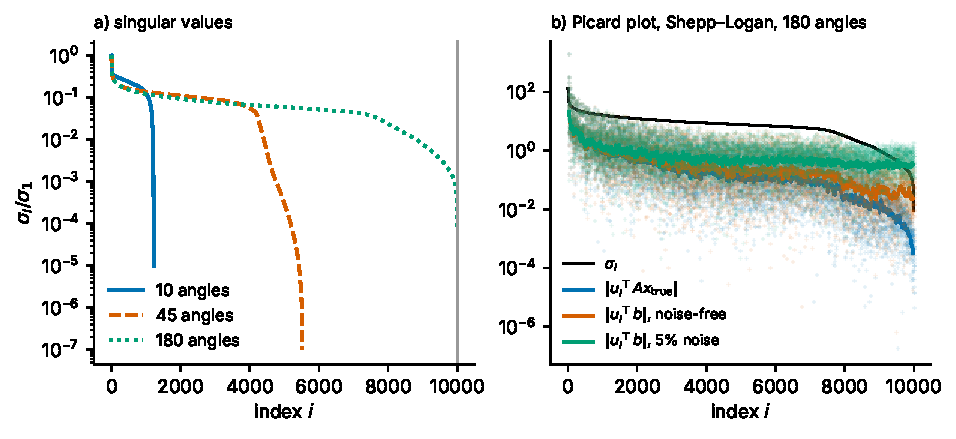
\includegraphics[width=\textwidth]{spectrum}
\caption{(a) Normalised singular values of the projection matrix for 10, 45 and 180 angles; the vertical line marks the number of unknowns. (b) Discrete Picard plot for the Shepp--Logan phantom with 180 angles: singular values and the coefficients $|u_i^\T b|$ of operator-consistent data $A\xt$, of the noise-free data simulated on the fine grid, and of data with 5\% noise (dots: individual coefficients; lines: moving geometric mean over 51 indices).}\label{fig:spectrum}
\end{figure}

The null-space fractions in the last two columns of \cref{tab:spectrum} turn \cref{prop:bound} into numbers. With 10 angles, 73\% of the norm of the digits phantom and 51\% of the norm of the Shepp--Logan phantom lie in the null space, and no method whose output lies in $\RR(A^\T)$ can achieve a smaller relative error. \Cref{fig:nullspace} shows the decomposition for the digits phantom: the visible part $P_{\RR}\xt$ is a blurred image overlaid by streaks along the measured directions, in which the digits can be located but not read, and the invisible part contains the strokes of the digits themselves together with a streak pattern that cancels the streaks of the visible part. The digits phantom has a larger null-space fraction than the Shepp--Logan phantom for every geometry, because its energy is concentrated in thin strokes, that is, at high spatial frequencies, which are exactly the frequencies left unsampled between the Fourier slices of \eqref{eq:slice}.

\begin{figure}[t]
\centering
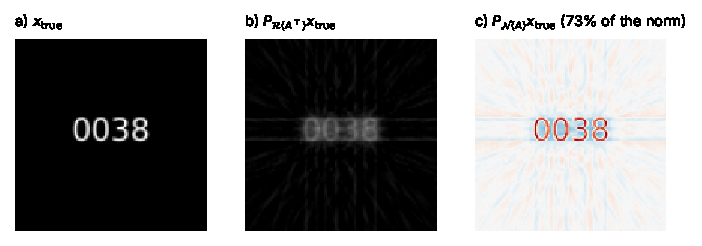
\includegraphics[width=0.8\textwidth]{nullspace}
\caption{Decomposition of the digits phantom for 10 angles into (b) its component in $\RR(A^\T)$, which is all that FBP, LSQR and Tikhonov regularisation can reconstruct, and (c) its component in the null space $\NN(A)$, which produces zero data.}\label{fig:nullspace}
\end{figure}

\subsection{Reconstruction accuracy and angular sampling}\label{sec:results-accuracy}

\Cref{fig:err} shows the relative error of the four methods with oracle parameters as a function of the number of angles, and \cref{tab:err} lists the values for 1\% noise together with the null-space bound. The results fall into three regimes. With few angles, 5 to 20, FBP is dominated by streak artefacts and has relative errors of 0.78 to 1.89 on the digits phantom and 0.42 to 1.17 on the Shepp--Logan phantom, errors above one meaning that the reconstruction is further from the truth than the zero image. LSQR and Tikhonov regularisation give almost identical errors in this regime, and these errors exceed the null-space bound by at most 0.03, for example 0.742 and 0.741 against the bound 0.734 for the digits phantom with 10 angles, and 0.521 and 0.519 against 0.511 for the Shepp--Logan phantom. The two methods thus reconstruct essentially the visible part $P_{\RR}\xt$ shown in \cref{fig:nullspace}(b), and they are limited by the measurement geometry, not by noise or by the choice of the parameter. TV regularisation is the only method that falls well below the bound, with 0.246 against 0.734 for the digits and 0.301 against 0.511 for the Shepp--Logan phantom at 10 angles, and its SSIM of 0.97 for the digits shows that it reconstructs the strokes that lie in the null space. The reconstructions in \cref{fig:recon} make the difference visible: with 10 angles the digits are legible only in the TV reconstruction, and even TV loses the low-contrast inner ellipses of the Shepp--Logan phantom, whose edges are weak compared with the outer skull.

\begin{figure}[t]
\centering
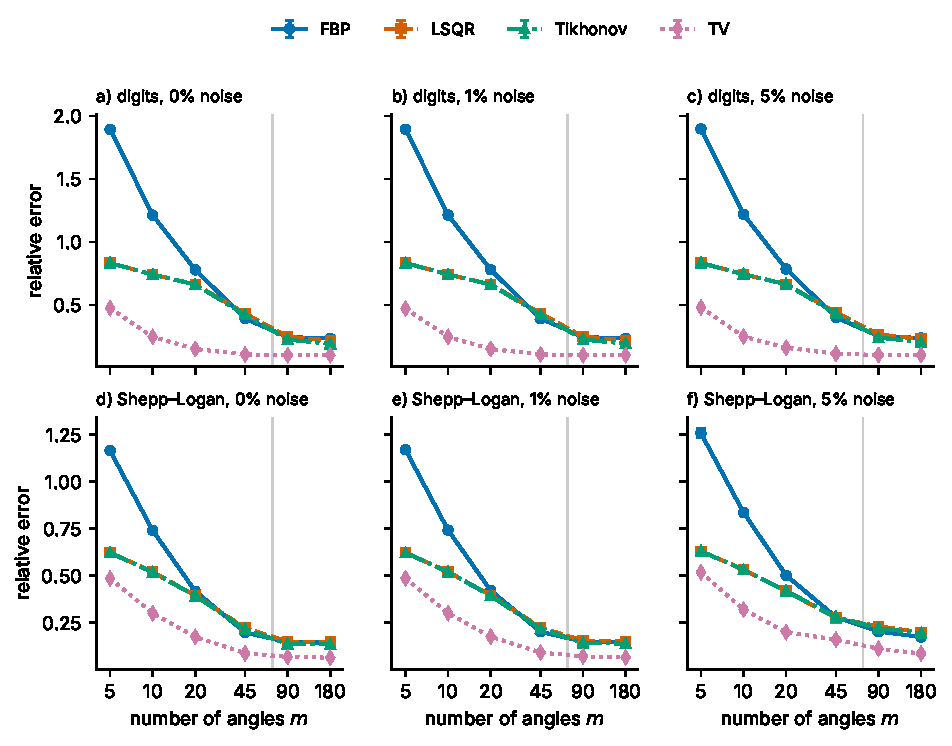
\includegraphics[width=\textwidth]{error_vs_angles}
\caption{Relative reconstruction error with oracle parameters against the number of angles for the two phantoms and three noise levels; error bars give the standard deviation over three noise realisations and are mostly smaller than the markers. The grey line at $m=n^2/n_d\approx70$ separates under- (left) from overdetermined (right) systems.}\label{fig:err}
\end{figure}

\begin{table}[t]
\centering
\caption{Relative error (SSIM in parentheses) with oracle parameters and 1\% noise, mean over three realisations, and the null-space bound of \cref{prop:bound}.}\label{tab:err}
\small
\begin{tabular}{lrccccc}
\toprule
Phantom & $m$ & bound & FBP & LSQR & Tikhonov & TV \\
\midrule
digits & 5 & 0.829 & 1.894 (0.05) & 0.832 (0.41) & 0.832 (0.40) & 0.471 (0.94) \\
 & 10 & 0.734 & 1.213 (0.08) & 0.742 (0.30) & 0.741 (0.31) & 0.246 (0.97) \\
 & 20 & 0.644 & 0.779 (0.10) & 0.662 (0.28) & 0.661 (0.28) & 0.150 (0.99) \\
 & 45 & 0.361 & 0.392 (0.23) & 0.432 (0.40) & 0.422 (0.39) & 0.107 (1.00) \\
 & 90 & 0 & 0.245 (0.76) & 0.248 (0.72) & 0.225 (0.76) & 0.101 (1.00) \\
 & 180 & 0 & 0.233 (0.94) & 0.217 (0.90) & 0.192 (0.83) & 0.101 (1.00) \\
\midrule
Shepp--Logan & 5 & 0.619 & 1.170 (0.34) & 0.623 (0.41) & 0.622 (0.41) & 0.486 (0.65) \\
 & 10 & 0.511 & 0.742 (0.39) & 0.521 (0.44) & 0.519 (0.44) & 0.301 (0.72) \\
 & 20 & 0.365 & 0.421 (0.50) & 0.396 (0.48) & 0.394 (0.47) & 0.176 (0.94) \\
 & 45 & 0.162 & 0.202 (0.63) & 0.225 (0.63) & 0.218 (0.63) & 0.091 (0.96) \\
 & 90 & 0 & 0.149 (0.81) & 0.154 (0.79) & 0.142 (0.78) & 0.071 (0.98) \\
 & 180 & 0 & 0.146 (0.89) & 0.150 (0.83) & 0.139 (0.80) & 0.066 (0.99) \\
\bottomrule
\end{tabular}
\end{table}

At 45 angles the gap between the linear methods and the bound widens to 0.06--0.07, because the singular values close to the tolerance now matter: components in $\RR(A^\T)$ that belong to very small singular values are visible in principle but cannot be recovered stably, which the bound does not account for. In this intermediate regime FBP becomes competitive with the algebraic methods, with 0.392 against 0.42--0.43 on the digits phantom and 0.202 against 0.22 on the Shepp--Logan phantom, and TV reaches 0.107 and 0.091. With 90 and 180 angles, where the systems are overdetermined, FBP, LSQR and Tikhonov regularisation agree to within 0.04, and the error of all three hardly changes between 90 and 180 angles. In this regime the accuracy is no longer limited by the angular sampling but by the discretisation, as \cref{sec:results-noise} shows. TV remains about twice as accurate as the linear methods, with 0.10 for the digits and 0.066--0.071 for the Shepp--Logan phantom, and its SSIM is 0.98--1.00 against 0.72--0.94 for the others. The distinction between over- and underdetermined systems, marked by the grey line in \cref{fig:err}, is not visible in any of the curves; the errors change smoothly across it, as would be expected from the spectral picture of \cref{sec:results-spectrum}.

\begin{figure}[t]
\centering
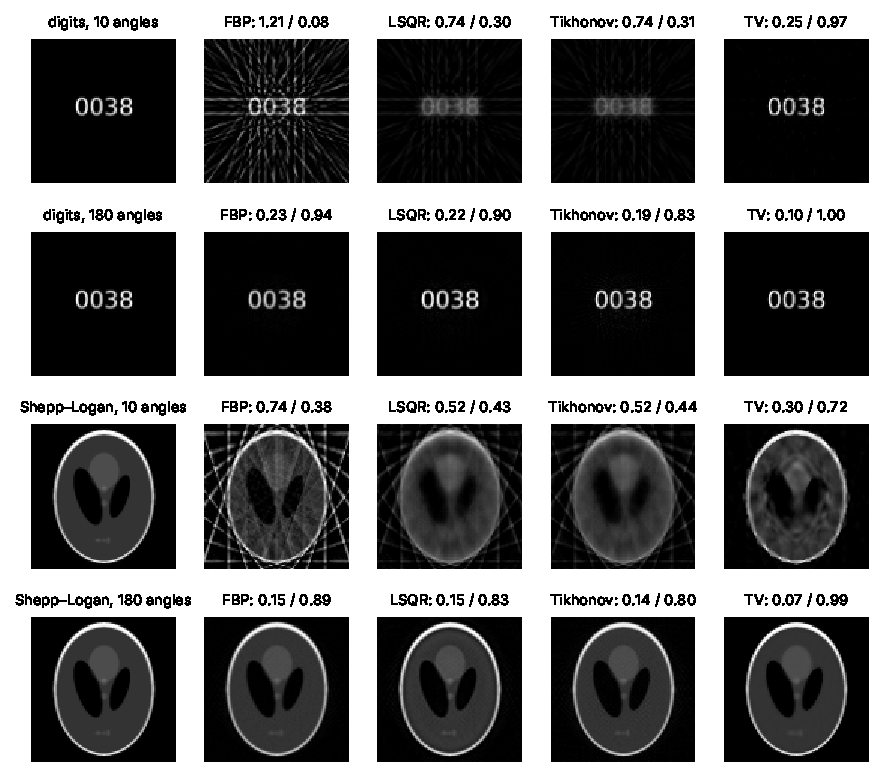
\includegraphics[width=\textwidth]{reconstructions}
\caption{Reconstructions with 1\% noise and oracle parameters for 10 angles (under\-determined) and 180 angles (overdetermined). Panel titles give relative error / SSIM.}\label{fig:recon}
\end{figure}

\subsection{Noise and model error}\label{sec:results-noise}

Increasing the noise from 0 to 1\% changes no relative error in \cref{fig:err} by more than 0.006, and increasing it to 5\% changes the errors of the digits phantom by at most 0.02. This insensitivity is explained by the model error of the simulated data, which is 6.0--8.1\% for the digits phantom and 2.0--3.1\% for the Shepp--Logan phantom, depending on $m$. A noise level of 1\% is thus small compared with the error that the discretisation itself introduces, and only for the Shepp--Logan phantom with 5\% noise does the noise exceed the model error. In this case the linear methods deteriorate noticeably at dense sampling, FBP from 0.146 to 0.175 and LSQR from 0.150 to 0.199 at 180 angles, while TV is less affected (0.066 to 0.087).

The Picard plot in \cref{fig:spectrum}(b) shows how the model error enters. For operator-consistent data $A\xt$ the coefficients $|u_i^\T b|$ decay with the singular values and fall well below them at the end of the spectrum, so that the discrete Picard condition holds. For the data simulated on the fine grid the coefficients level off at about $5\times10^{-2}$ in the second half of the spectrum, and with 5\% noise at about $0.3$; in both cases they exceed the singular values in the last few hundred indices, where the unregularised solution \eqref{eq:pinv} is therefore dominated by data error. The model error thus behaves like an additional noise component, although it is neither random nor independent of the object. A related consequence concerns the residual: since the fine-grid data are not in $\RR(A)$, the least-squares residual of the noise-free data has the floor $\|(I-AA^+)b_0\|/\|b_0\|$, which is 0.5--0.9\% for the digits phantom and 0.09--0.56\% for the Shepp--Logan phantom in the overdetermined case. These floors are of the same order as a noise level of 1\%, which has direct consequences for the choice of the regularisation parameter.

\subsection{Parameter sensitivity and the discrepancy principle}\label{sec:results-param}

\Cref{fig:params} shows the relative error of the three regularised methods as a function of their parameters for the digits phantom. LSQR exhibits the semi-convergence described in \cref{sec:methods-lsqr}: the error reaches its minimum after 4 to 11 iterations and then increases, slowly with 10 angles, where it saturates near one, and steeply with 180 angles, where it exceeds one after about 200 iterations although the noise level is only 1\%. The steep increase at 180 angles is caused by the small singular values at the end of the spectrum, which are reached by the Krylov iteration once the larger ones have converged, and by the model error that their coefficients carry. The Tikhonov curves have a similar shape, with a broad minimum around $\tilde\lambda\approx0.3$--1, and their minima are as low as those of LSQR or slightly lower. The TV curves are remarkably uniform: for all three angle counts and both noise levels the optimum lies at $\tilde\lambda=0.03$, which suggests that the scaling $\lambda=m\tilde\lambda$ captures the dependence on the geometry. The minimum is nevertheless narrow: one grid step, a factor of about three, away from the optimum the error grows by 60--130\% for 45 and 180 angles, so that TV is less forgiving of a poorly chosen parameter than the two linear methods.

\begin{figure}[t]
\centering
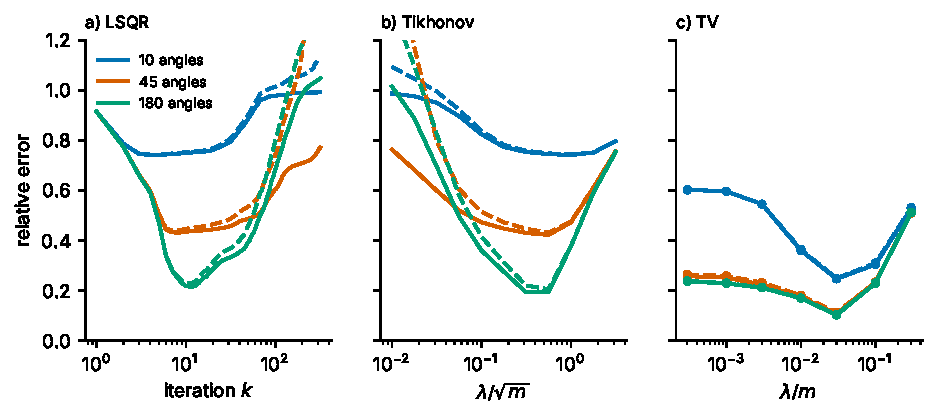
\includegraphics[width=\textwidth]{parameter_curves}
\caption{Relative error of the digits phantom reconstructions against (a) the LSQR iteration count, (b) the scaled Tikhonov parameter and (c) the scaled TV parameter, for 10, 45 and 180 angles with 1\% (solid) and 5\% (dashed) noise; means over three realisations.}\label{fig:params}
\end{figure}

\Cref{tab:discrepancy} compares the oracle with the discrepancy principle. When the threshold is based on the noise level alone, $\delta=\|e\|$, the principle fails in most cases with 1\% noise. For the digits phantom the threshold is below the attainable residual for 10 and 180 angles, the iteration is never stopped, and LSQR and Tikhonov return nearly unregularised solutions with relative errors around one, about five times the oracle error at 180 angles. For TV the threshold is never reached for the digits phantom, and the least regularised element of the grid has errors of 0.24--0.60, about 2.4 times the oracle error. With 5\% noise the noise dominates the total error and the noise-based principle works much better, with errors within 0.015 of the oracle for LSQR and Tikhonov at 10 and 45 angles, although TV still fails for the digits phantom because its residual at moderate $\lambda$ remains above the threshold. When the threshold is based on the total error, $\delta=\|b-A\xt\|$, the discrepancy principle comes within 0.01 of the oracle error in almost all cases, the exceptions being Tikhonov at 180 angles, where the error grows from 0.139 to 0.157 and from 0.205 to 0.219, and TV for the Shepp--Logan phantom with 10 angles. The principle occasionally even improves on the oracle by a small margin, because it chooses the parameter separately for every noise realisation and, for LSQR, from every iteration rather than from the grid of 16 iteration counts. The conclusion is that the discrepancy principle is reliable for this problem if, and only if, its threshold accounts for the model error.

\begin{table}[t]
\centering
\caption{Relative error with the parameter chosen by the oracle and by the discrepancy principle with threshold $1.05\,\delta$ based on the noise level ($\delta=\|e\|$) or on the total data error ($\delta=\|b-A\xt\|$); mean over three realisations. An asterisk marks cases in which the threshold was not attained for any realisation and the least regularised parameter was returned.}\label{tab:discrepancy}
\small
\setlength{\tabcolsep}{4pt}
\begin{tabular}{lrr ccc ccc ccc}
\toprule
 & & & \multicolumn{3}{c}{LSQR} & \multicolumn{3}{c}{Tikhonov} & \multicolumn{3}{c}{TV} \\
\cmidrule(lr){4-6}\cmidrule(lr){7-9}\cmidrule(lr){10-12}
Phantom & $m$ & $\eta$ & oracle & $\|e\|$ & total & oracle & $\|e\|$ & total & oracle & $\|e\|$ & total \\
\midrule
digits & 10 & 1\% & 0.742 & 0.992$^\ast$ & 0.742 & 0.741 & 0.987$^\ast$ & 0.741 & 0.246 & 0.602$^\ast$ & 0.246 \\
 & 45 & 1\% & 0.432 & 0.515 & 0.431 & 0.422 & 0.520 & 0.422 & 0.107 & 0.257$^\ast$ & 0.107 \\
 & 180 & 1\% & 0.217 & 1.048$^\ast$ & 0.215 & 0.192 & 1.015$^\ast$ & 0.192 & 0.101 & 0.236$^\ast$ & 0.101 \\
Shepp--Logan & 10 & 1\% & 0.521 & 0.521 & 0.522 & 0.519 & 0.520 & 0.519 & 0.301 & 0.426 & 0.384 \\
 & 45 & 1\% & 0.225 & 0.236 & 0.224 & 0.218 & 0.243 & 0.226 & 0.091 & 0.456 & 0.091 \\
 & 180 & 1\% & 0.150 & 0.266 & 0.149 & 0.139 & 0.267 & 0.157 & 0.066 & 0.306$^\ast$ & 0.066 \\
\midrule
digits & 10 & 5\% & 0.743 & 0.747 & 0.743 & 0.743 & 0.748 & 0.743 & 0.248 & 0.601$^\ast$ & 0.248 \\
 & 45 & 5\% & 0.440 & 0.445 & 0.440 & 0.432 & 0.446 & 0.432 & 0.112 & 0.264$^\ast$ & 0.112 \\
 & 180 & 5\% & 0.229 & 0.293 & 0.229 & 0.205 & 0.312 & 0.219 & 0.103 & 0.238$^\ast$ & 0.103 \\
Shepp--Logan & 10 & 5\% & 0.533 & 0.533 & 0.533 & 0.532 & 0.532 & 0.532 & 0.320 & 0.320 & 0.320 \\
 & 45 & 5\% & 0.276 & 0.276 & 0.276 & 0.280 & 0.280 & 0.280 & 0.161 & 0.161 & 0.170 \\
 & 180 & 5\% & 0.199 & 0.197 & 0.199 & 0.193 & 0.238 & 0.193 & 0.087 & 0.087 & 0.087 \\
\bottomrule
\end{tabular}
\end{table}

\subsection{The inverse crime}\label{sec:results-crime}

To measure how much the inverse crime would have distorted the comparison, we repeated the experiments for 10, 45 and 180 angles with data $b=A\xt+e$ generated by the reconstruction operator itself. \Cref{tab:crime} shows that the effect depends strongly on the method and on the size of the model error. For the digits phantom, whose model error is large, the criminal data reduce the TV error from 0.246 to 0.092 at 10 angles and from 0.101 to 0.013 at 180 angles with 1\% noise, that is, by a factor of almost eight, and the errors of LSQR and Tikhonov at 180 angles fall from 0.217 and 0.192 to 0.125. At 10 angles, in contrast, LSQR and Tikhonov hardly benefit, because their error is fixed by the null-space bound, which does not depend on the data. FBP behaves in the opposite way at dense sampling, with errors of 0.313 instead of 0.233 at 180 angles: the pixel-driven forward projection of the coarse image contains the high-frequency artefacts mentioned in \cref{sec:discrete-matrix}, which the ramp filter amplifies, whereas the fine-grid data resemble true line integrals more closely. For the Shepp--Logan phantom, whose model error of 2--3\% is comparable with the noise, the effects are smaller and of either sign. Had we used criminal data, we would have concluded that TV reconstructs the digits phantom almost perfectly from 45 angles and that the algebraic methods are clearly superior to FBP at 180 angles; neither conclusion survives a realistic data model.

\begin{table}[t]
\centering
\caption{Relative error with oracle parameters for data generated with the reconstruction operator ($b=A\xt+e$, ``crime'') and with the fine-grid data model (``fine''); mean over three realisations.}\label{tab:crime}
\small
\setlength{\tabcolsep}{4.5pt}
\begin{tabular}{lrr cc cc cc cc}
\toprule
 & & & \multicolumn{2}{c}{FBP} & \multicolumn{2}{c}{LSQR} & \multicolumn{2}{c}{Tikhonov} & \multicolumn{2}{c}{TV} \\
\cmidrule(lr){4-5}\cmidrule(lr){6-7}\cmidrule(lr){8-9}\cmidrule(lr){10-11}
Phantom & $m$ & $\eta$ & crime & fine & crime & fine & crime & fine & crime & fine \\
\midrule
digits & 10 & 1\% & 1.013 & 1.213 & 0.736 & 0.742 & 0.736 & 0.741 & 0.092 & 0.246 \\
 & 45 & 1\% & 0.388 & 0.392 & 0.409 & 0.432 & 0.409 & 0.422 & 0.016 & 0.107 \\
 & 180 & 1\% & 0.313 & 0.233 & 0.125 & 0.217 & 0.125 & 0.192 & 0.013 & 0.101 \\
Shepp--Logan & 10 & 1\% & 0.642 & 0.742 & 0.515 & 0.521 & 0.515 & 0.519 & 0.219 & 0.301 \\
 & 45 & 1\% & 0.220 & 0.202 & 0.207 & 0.225 & 0.207 & 0.218 & 0.101 & 0.091 \\
 & 180 & 1\% & 0.194 & 0.146 & 0.095 & 0.150 & 0.094 & 0.139 & 0.049 & 0.066 \\
\midrule
digits & 10 & 5\% & 1.022 & 1.218 & 0.741 & 0.743 & 0.741 & 0.743 & 0.168 & 0.248 \\
 & 45 & 5\% & 0.396 & 0.401 & 0.425 & 0.440 & 0.428 & 0.432 & 0.069 & 0.112 \\
 & 180 & 5\% & 0.316 & 0.237 & 0.189 & 0.229 & 0.198 & 0.205 & 0.037 & 0.103 \\
Shepp--Logan & 10 & 5\% & 0.746 & 0.836 & 0.531 & 0.533 & 0.532 & 0.532 & 0.332 & 0.320 \\
 & 45 & 5\% & 0.293 & 0.280 & 0.288 & 0.276 & 0.289 & 0.280 & 0.169 & 0.161 \\
 & 180 & 5\% & 0.217 & 0.175 & 0.206 & 0.199 & 0.220 & 0.193 & 0.116 & 0.087 \\
\bottomrule
\end{tabular}
\end{table}

\subsection{Filter windows and limited-angle data}\label{sec:results-supp}

The results so far used FBP with the Ram--Lak filter, which is the natural choice for comparison because it involves no smoothing beyond the band limit of the detector. \Cref{tab:windows} shows that apodising windows change the picture in a way that depends on the angular sampling. With 10 angles the Hann window reduces the relative error of FBP from 1.21 to 0.83 for the digits phantom and from 0.74 to 0.56 for the Shepp--Logan phantom, because it suppresses the high-frequency streaks that dominate the error, but the improved FBP is still worse than LSQR and Tikhonov regularisation at the same sampling. With 180 angles the Hann window doubles the relative error, from 0.233 to 0.469 and from 0.146 to 0.290, because it blurs edges that the dense data would allow to be resolved, although the SSIM hardly changes or even improves slightly. The Shepp--Logan window lies in between. A window thus acts as a crude regularisation parameter for FBP, and the best window depends on the number of angles and on the noise level in the same way as the regularisation parameters of the other methods; in particular, the Hann window is never the best choice in terms of relative error at 180 angles, whereas it is the best choice at 10 angles. The discrepancy between relative error and SSIM for the smoothing windows also illustrates that the two measures reward different properties: SSIM is insensitive to a uniform blur of a high-contrast image as long as the structure is preserved, while the relative error penalises the displaced intensity at every edge.

\begin{table}[t]
\centering
\caption{Relative error (SSIM in parentheses) of FBP with three filter windows, mean over three noise realisations.}\label{tab:windows}
\small
\begin{tabular}{lrr ccc}
\toprule
Phantom & $m$ & $\eta$ & Ram--Lak & Shepp--Logan & Hann \\
\midrule
digits & 10 & 1\% & 1.213 (0.08) & 1.109 (0.08) & 0.830 (0.11) \\
 & 45 & 1\% & 0.392 (0.23) & 0.385 (0.30) & 0.481 (0.69) \\
 & 180 & 1\% & 0.233 (0.94) & 0.281 (0.95) & 0.469 (0.96) \\
 & 10 & 5\% & 1.218 (0.07) & 1.112 (0.08) & 0.832 (0.11) \\
 & 45 & 5\% & 0.401 (0.22) & 0.391 (0.28) & 0.482 (0.67) \\
 & 180 & 5\% & 0.237 (0.88) & 0.284 (0.91) & 0.470 (0.95) \\
\midrule
Shepp--Logan & 10 & 1\% & 0.742 (0.39) & 0.688 (0.41) & 0.559 (0.45) \\
 & 45 & 1\% & 0.202 (0.63) & 0.208 (0.65) & 0.293 (0.79) \\
 & 180 & 1\% & 0.146 (0.89) & 0.174 (0.91) & 0.290 (0.90) \\
 & 10 & 5\% & 0.836 (0.26) & 0.758 (0.28) & 0.579 (0.37) \\
 & 45 & 5\% & 0.280 (0.43) & 0.261 (0.46) & 0.302 (0.65) \\
 & 180 & 5\% & 0.175 (0.64) & 0.191 (0.70) & 0.293 (0.83) \\
\bottomrule
\end{tabular}
\end{table}

The second form of incompleteness discussed in \cref{sec:radon-illposed} is a restricted angular range. We kept the number of angles at $m=90$ and distributed them uniformly over $[0,\Phi)$ for $\Phi\in\{180^\circ,150^\circ,120^\circ,90^\circ\}$, with 1\% noise and oracle parameters on the same grids as before, so that the size of the system stays the same while the double wedge of unmeasured Fourier directions grows. \Cref{tab:limited} shows that all methods deteriorate much more than the size of the system would suggest. The error of the three linear methods on the digits phantom grows from 0.23--0.25 for the full range to 0.42--0.44 at $150^\circ$ and to 0.63--0.67 at $90^\circ$, which is close to the error obtained from 20 angles over the full range (0.66), although the number of measurements is four and a half times larger. TV remains the most accurate method, but its advantage shrinks: its error grows by a factor of four, from 0.101 to 0.429, which is worse than its error of 0.246 with only 10 angles over the full range, and for the Shepp--Logan phantom at $90^\circ$ it is only 10\% below that of Tikhonov regularisation. This agrees with the microlocal picture: an edge whose normal direction lies in the missing wedge produces no singularity in the data, so that a piecewise constant prior can extend edges that are partly visible but cannot recover the orientation information that is missing altogether \citep{quinto1993}. In the sparse-view case, in contrast, every edge direction is measured up to the angular spacing, which is why TV can close the gaps so effectively there.

\begin{table}[t]
\centering
\caption{Relative error (SSIM in parentheses) for $m=90$ angles distributed over $[0,\Phi)$ with 1\% noise and oracle parameters, mean over three realisations.}\label{tab:limited}
\small
\begin{tabular}{lr cccc}
\toprule
Phantom & $\Phi$ & FBP & LSQR & Tikhonov & TV \\
\midrule
digits & $180^\circ$ & 0.245 (0.76) & 0.248 (0.72) & 0.225 (0.76) & 0.101 (1.00) \\
 & $150^\circ$ & 0.424 (0.67) & 0.436 (0.63) & 0.420 (0.66) & 0.155 (1.00) \\
 & $120^\circ$ & 0.521 (0.68) & 0.524 (0.63) & 0.508 (0.66) & 0.270 (0.99) \\
 & $90^\circ$ & 0.668 (0.63) & 0.633 (0.49) & 0.627 (0.55) & 0.429 (0.97) \\
\midrule
Shepp--Logan & $180^\circ$ & 0.149 (0.81) & 0.154 (0.79) & 0.142 (0.78) & 0.071 (0.98) \\
 & $150^\circ$ & 0.371 (0.66) & 0.326 (0.66) & 0.316 (0.64) & 0.248 (0.82) \\
 & $120^\circ$ & 0.516 (0.60) & 0.439 (0.58) & 0.426 (0.57) & 0.368 (0.79) \\
 & $90^\circ$ & 0.624 (0.56) & 0.529 (0.44) & 0.521 (0.49) & 0.469 (0.69) \\
\bottomrule
\end{tabular}
\end{table}

\subsection{Convergence and computational cost}\label{sec:results-cost}

All TV results above were obtained with 600 iterations of the primal--dual algorithm, and \cref{fig:tvconv} shows how far these iterates are from convergence. For each phantom with 10 and 180 angles we ran 3{,}000 iterations with the oracle parameter and 1\% noise and recorded the objective and the relative error every ten iterations. With 180 angles the objective at iteration 600 is within 0.3\% (digits) and 1.3\% (Shepp--Logan) of its value after 3{,}000 iterations, and the relative error has settled at 0.102 and 0.066, which differ from the values at 3{,}000 iterations by at most 0.002. With 10 angles convergence is markedly slower, as one would expect when the data term leaves a large null space on which the objective is determined by the TV term alone and is therefore flat along many directions. For the digits phantom the error at 600 iterations, 0.247, is still within 0.004 of the error at 3{,}000 iterations, but for the Shepp--Logan phantom the objective at 600 iterations is 17\% above its final value and the error decreases further from 0.299 to 0.259. The TV errors reported for the Shepp--Logan phantom with few angles are therefore slightly pessimistic, and the advantage of TV over the linear methods in this regime is, if anything, understated.

\begin{figure}[t]
\centering
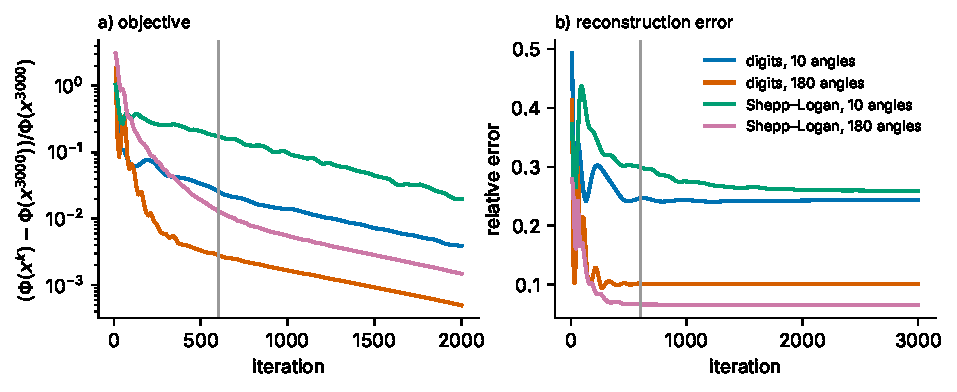
\includegraphics[width=\textwidth]{tv_convergence}
\caption{Convergence of the primal--dual algorithm for TV regularisation with the oracle parameter and 1\% noise: (a) relative distance of the objective from its value after 3{,}000 iterations, (b) relative reconstruction error. The vertical lines mark the 600 iterations used in all other experiments.}\label{fig:tvconv}
\end{figure}

The cost of the methods differs by three orders of magnitude. On a single core of a Linux virtual machine, for 180 angles, one product with $A$ followed by one with $A^\T$ takes 13\,ms, FBP takes 9\,ms, LSQR with the oracle count of 10 iterations 0.14\,s, Tikhonov regularisation by damped LSQR 1.9\,s, and 600 iterations of the primal--dual algorithm 8.5\,s. Measured in products with $A$ and $A^\T$, which dominate all iterative methods, FBP costs less than one product pair, LSQR about ten, Tikhonov regularisation up to 500, because damped LSQR has to converge rather than stop early, and TV 600 plus the gradient operations. These costs refer to a single parameter value; the oracle and the discrepancy principle require the whole grid, which for LSQR comes at no extra cost, since all iteration counts are produced by one run, but multiplies the cost of Tikhonov and TV regularisation by the number of grid points.

%% ==================================================================
\section{Discussion}\label{sec:discussion}

The experiments support a simple account of sparse-view reconstruction in which the size of the linear system plays a minor role. What determines the attainable accuracy of a linear method is the part of the object that the measurements do not see, and \cref{prop:bound} together with \cref{tab:spectrum} predicts the error plateau of LSQR and Tikhonov regularisation at 5 to 20 angles to within 0.03. In this regime the regularisation parameter, the noise level and the choice between the two methods are nearly irrelevant, since all of them act only on $\RR(A^\T)$. When the null space shrinks, the singular values take over, and the effective number of well-determined directions in \cref{tab:spectrum} describes the behaviour of the overdetermined system with 90 angles better than its formal rank. A method can only do better than the bound by putting something into the null space, and TV does so successfully for both phantoms because the null-space components of a piecewise constant image are largely determined by the requirement that the image be piecewise constant. The quality of sparse-view reconstruction is therefore primarily a question of prior information, which is also the conclusion of the phase-diagram studies of \citep{jorgensen2015}; our contribution is to make the role of the null space quantitative for a concrete geometry. The second message of the experiments is that the discretisation error is not a detail: at a noise level of 1\% it is the dominant data error, it limits the accuracy of all methods at dense sampling, it determines whether the discrepancy principle works, and ignoring it through the inverse crime would have overstated the accuracy of TV by up to a factor of eight.

These conclusions are subject to several limitations. Both phantoms are piecewise constant, which is exactly the class of images that TV favours, and natural images with texture or smooth gradients would reduce the advantage of TV and expose its staircasing; higher-order penalties such as total generalised variation \citep{bredies2010} address the latter. The oracle parameters are not available in practice, and although the discrepancy principle with the total data error comes close to them, it requires an estimate of the model error, which is difficult to obtain without knowledge of the object; rules that do not need $\delta$, such as generalised cross-validation \citep{golub1979} or the L-curve \citep{hansen1992}, may then be preferable and should be evaluated with the same data model. The noise model is additive, Gaussian and white with a prescribed relative norm, whereas measured CT data follow a Poisson law after the logarithmic transformation and call for weighted least-squares data terms \citep{herman2009}. The grid of $100\times100$ pixels was chosen so that the spectral analysis could be carried out exactly; at clinical resolutions only partial spectral information can be computed, but the bound of \cref{prop:bound} can still be evaluated for a test object by an iterative solver applied to the consistent data $A\xt$. Finally, the projector is a simple pixel-driven model, and ray-driven \citep{siddon1985} or distance-driven \citep{deman2004} projectors would reduce the model error that limits all methods at dense sampling and would change the balance between FBP and the algebraic methods seen in \cref{tab:crime}.

The same framework suggests several extensions. Since \cref{prop:bound} characterises everything that methods with output in $\RR(A^\T)$ cannot do, it provides a natural baseline for learned reconstruction methods \citep{jin2017,adler2018} and for plug-and-play priors \citep{venkatakrishnan2013}, which can be evaluated by how much of the null-space component they recover and how reliably they do so. Algebraic methods with non-negativity constraints, such as ART \citep{gordon1970} and SART \citep{andersen1984}, do not produce outputs in $\RR(A^\T)$ either and would be interesting intermediates between the linear methods and TV. The limited-angle experiment of \cref{sec:results-supp} indicates that the structure of the null space matters as much as its dimension, and a direction-dependent analysis in the spirit of microlocal analysis \citep{quinto1993} could explain which edges are lost for a given angular range. Finally, the influence of the model error on the parameter choice suggests that parameter choice rules for tomography should be tested with data generated on finer grids, or with continuous phantoms projected analytically, as a matter of course.

%% ==================================================================
\section{Conclusions}\label{sec:conclusions}

We have studied parallel-beam image reconstruction from 5 to 180 projection angles, a range over which the discretised problem passes from strongly underdetermined to overdetermined, by combining an exact spectral analysis of the projection matrices with a systematic comparison of filtered back-projection, LSQR, Tikhonov regularisation and TV regularisation on data free of the inverse crime. The analysis shows that with 10 angles 88\% of the image space is invisible to the measurements, and that every method whose output lies in the range of $A^\T$, including FBP, LSQR and Tikhonov regularisation, is bounded below by the fraction of the object in the null space, 0.73 for the digits phantom and 0.51 for the Shepp--Logan phantom; the observed errors of LSQR and Tikhonov regularisation lie within 0.03 of this bound. TV regularisation, which fills the null space with piecewise constant structure, reduces the error to a third for the digits phantom and to about 60\% of the bound for the Shepp--Logan phantom. With many angles the system is overdetermined but remains ill-conditioned, the three linear methods perform alike, and their accuracy is limited by the discretisation error of the projector, which at 1\% noise exceeds the noise itself, causes the discrepancy principle to fail unless it is included in the error estimate, and would have been concealed by the inverse crime. Sparse-view reconstruction is therefore governed by the null space and the singular values of the projection matrix and by the prior information used to fill the null space, rather than by whether the linear system has more or fewer equations than unknowns.

\begingroup
\small
\begin{thebibliography}{99}
\bibitem[Acar and Vogel(1994)]{acar1994} R.~Acar and C.~R. Vogel. Analysis of bounded variation penalty methods for ill-posed problems. \emph{Inverse Problems}, 10(6):1217--1229, 1994.
\bibitem[Adler and {\"O}ktem(2018)]{adler2018} J.~Adler and O.~{\"O}ktem. Learned primal-dual reconstruction. \emph{IEEE Transactions on Medical Imaging}, 37(6):1322--1332, 2018.
\bibitem[Andersen and Kak(1984)]{andersen1984} A.~H. Andersen and A.~C. Kak. Simultaneous algebraic reconstruction technique ({SART}): a superior implementation of the {ART} algorithm. \emph{Ultrasonic Imaging}, 6(1):81--94, 1984.
\bibitem[Bj{\"o}rck(1996)]{bjorck1996} {\AA}.~Bj{\"o}rck. \emph{Numerical Methods for Least Squares Problems}. SIAM, Philadelphia, 1996.
\bibitem[Bredies et~al.(2010)]{bredies2010} K.~Bredies, K.~Kunisch, and T.~Pock. Total generalized variation. \emph{SIAM Journal on Imaging Sciences}, 3(3):492--526, 2010.
\bibitem[Cand{\`e}s et~al.(2006)]{candes2006} E.~J. Cand{\`e}s, J.~Romberg, and T.~Tao. Robust uncertainty principles: exact signal reconstruction from highly incomplete frequency information. \emph{IEEE Transactions on Information Theory}, 52(2):489--509, 2006.
\bibitem[Chambolle(2004)]{chambolle2004} A.~Chambolle. An algorithm for total variation minimization and applications. \emph{Journal of Mathematical Imaging and Vision}, 20(1--2):89--97, 2004.
\bibitem[Chambolle and Pock(2011)]{chambolle2011} A.~Chambolle and T.~Pock. A first-order primal--dual algorithm for convex problems with applications to imaging. \emph{Journal of Mathematical Imaging and Vision}, 40(1):120--145, 2011.
\bibitem[Chambolle and Pock(2016)]{chambolle2016} A.~Chambolle and T.~Pock. An introduction to continuous optimization for imaging. \emph{Acta Numerica}, 25:161--319, 2016.
\bibitem[Colton and Kress(1998)]{colton1998} D.~Colton and R.~Kress. \emph{Inverse Acoustic and Electromagnetic Scattering Theory}. 2nd ed., Springer, Berlin, 1998.
\bibitem[Davison(1983)]{davison1983} M.~E. Davison. The ill-conditioned nature of the limited angle tomography problem. \emph{SIAM Journal on Applied Mathematics}, 43(2):428--448, 1983.
\bibitem[De~Man and Basu(2004)]{deman2004} B.~De~Man and S.~Basu. Distance-driven projection and backprojection in three dimensions. \emph{Physics in Medicine and Biology}, 49(11):2463--2475, 2004.
\bibitem[Engl et~al.(1996)]{engl1996} H.~W. Engl, M.~Hanke, and A.~Neubauer. \emph{Regularization of Inverse Problems}. Kluwer, Dordrecht, 1996.
\bibitem[Golub et~al.(1979)]{golub1979} G.~H. Golub, M.~Heath, and G.~Wahba. Generalized cross-validation as a method for choosing a good ridge parameter. \emph{Technometrics}, 21(2):215--223, 1979.
\bibitem[Gordon et~al.(1970)]{gordon1970} R.~Gordon, R.~Bender, and G.~T. Herman. Algebraic reconstruction techniques ({ART}) for three-dimensional electron microscopy and {X}-ray photography. \emph{Journal of Theoretical Biology}, 29(3):471--481, 1970.
\bibitem[Hanke(1995)]{hanke1995} M.~Hanke. \emph{Conjugate Gradient Type Methods for Ill-Posed Problems}. Longman, Harlow, 1995.
\bibitem[Hansen(1990)]{hansen1990} P.~C. Hansen. The discrete {P}icard condition for discrete ill-posed problems. \emph{BIT Numerical Mathematics}, 30(4):658--672, 1990.
\bibitem[Hansen(1992)]{hansen1992} P.~C. Hansen. Analysis of discrete ill-posed problems by means of the {L}-curve. \emph{SIAM Review}, 34(4):561--580, 1992.
\bibitem[Hansen(2010)]{hansen2010} P.~C. Hansen. \emph{Discrete Inverse Problems: Insight and Algorithms}. SIAM, Philadelphia, 2010.
\bibitem[Hansen and J{\o}rgensen(2018)]{hansen2018} P.~C. Hansen and J.~S. J{\o}rgensen. {AIR Tools II}: algebraic iterative reconstruction methods, improved implementation. \emph{Numerical Algorithms}, 79(1):107--137, 2018.
\bibitem[Herman(2009)]{herman2009} G.~T. Herman. \emph{Fundamentals of Computerized Tomography: Image Reconstruction from Projections}. 2nd ed., Springer, London, 2009.
\bibitem[Jin et~al.(2017)]{jin2017} K.~H. Jin, M.~T. McCann, E.~Froustey, and M.~Unser. Deep convolutional neural network for inverse problems in imaging. \emph{IEEE Transactions on Image Processing}, 26(9):4509--4522, 2017.
\bibitem[J{\o}rgensen and Sidky(2015)]{jorgensen2015} J.~S. J{\o}rgensen and E.~Y. Sidky. How little data is enough? {P}hase-diagram analysis of sparsity-regularized {X}-ray computed tomography. \emph{Philosophical Transactions of the Royal Society A}, 373(2043):20140387, 2015.
\bibitem[Kaipio and Somersalo(2005)]{kaipio2005} J.~Kaipio and E.~Somersalo. \emph{Statistical and Computational Inverse Problems}. Springer, New York, 2005.
\bibitem[Kak and Slaney(2001)]{kak2001} A.~C. Kak and M.~Slaney. \emph{Principles of Computerized Tomographic Imaging}. SIAM, Philadelphia, 2001.
\bibitem[Louis(1984)]{louis1984} A.~K. Louis. Orthogonal function series expansions and the null space of the {R}adon transform. \emph{SIAM Journal on Mathematical Analysis}, 15(3):621--633, 1984.
\bibitem[Morozov(1966)]{morozov1966} V.~A. Morozov. On the solution of functional equations by the method of regularization. \emph{Soviet Mathematics Doklady}, 7:414--417, 1966.
\bibitem[Natterer(2001)]{natterer2001} F.~Natterer. \emph{The Mathematics of Computerized Tomography}. SIAM, Philadelphia, 2001.
\bibitem[Paige and Saunders(1982)]{paige1982} C.~C. Paige and M.~A. Saunders. {LSQR}: an algorithm for sparse linear equations and sparse least squares. \emph{ACM Transactions on Mathematical Software}, 8(1):43--71, 1982.
\bibitem[Quinto(1993)]{quinto1993} E.~T. Quinto. Singularities of the {X}-ray transform and limited data tomography in $\mathbb{R}^2$ and $\mathbb{R}^3$. \emph{SIAM Journal on Mathematical Analysis}, 24(5):1215--1225, 1993.
\bibitem[Radon(1917)]{radon1917} J.~Radon. {\"U}ber die {B}estimmung von {F}unktionen durch ihre {I}ntegralwerte l{\"a}ngs gewisser {M}annigfaltigkeiten. \emph{Berichte {\"u}ber die Verhandlungen der S{\"a}chsischen Akademie der Wissenschaften zu Leipzig, Mathematisch-Physische Klasse}, 69:262--277, 1917.
\bibitem[Rudin et~al.(1992)]{rudin1992} L.~I. Rudin, S.~Osher, and E.~Fatemi. Nonlinear total variation based noise removal algorithms. \emph{Physica D}, 60(1--4):259--268, 1992.
\bibitem[Shepp and Logan(1974)]{shepp1974} L.~A. Shepp and B.~F. Logan. The {F}ourier reconstruction of a head section. \emph{IEEE Transactions on Nuclear Science}, 21(3):21--43, 1974.
\bibitem[Sidky and Pan(2008)]{sidky2008} E.~Y. Sidky and X.~Pan. Image reconstruction in circular cone-beam computed tomography by constrained, total-variation minimization. \emph{Physics in Medicine and Biology}, 53(17):4777--4807, 2008.
\bibitem[Sidky et~al.(2012)]{sidky2012} E.~Y. Sidky, J.~H. J{\o}rgensen, and X.~Pan. Convex optimization problem prototyping for image reconstruction in computed tomography with the {C}hambolle--{P}ock algorithm. \emph{Physics in Medicine and Biology}, 57(10):3065--3091, 2012.
\bibitem[Siddon(1985)]{siddon1985} R.~L. Siddon. Fast calculation of the exact radiological path for a three-dimensional {CT} array. \emph{Medical Physics}, 12(2):252--255, 1985.
\bibitem[Smith et~al.(1977)]{smith1977} K.~T. Smith, D.~C. Solmon, and S.~L. Wagner. Practical and mathematical aspects of the problem of reconstructing objects from radiographs. \emph{Bulletin of the American Mathematical Society}, 83(6):1227--1270, 1977.
\bibitem[Venkatakrishnan et~al.(2013)]{venkatakrishnan2013} S.~V. Venkatakrishnan, C.~A. Bouman, and B.~Wohlberg. Plug-and-play priors for model based reconstruction. In \emph{IEEE Global Conference on Signal and Information Processing}, pages 945--948, 2013.
\bibitem[Wang et~al.(2004)]{wang2004} Z.~Wang, A.~C. Bovik, H.~R. Sheikh, and E.~P. Simoncelli. Image quality assessment: from error visibility to structural similarity. \emph{IEEE Transactions on Image Processing}, 13(4):600--612, 2004.
\end{thebibliography}
\endgroup
\end{document}
